\documentclass[12pt]{article}
\usepackage[utf8]{inputenc}
\usepackage{amsmath}
\usepackage{amsfonts}
\usepackage{graphicx}
\usepackage[backend=biber, style=numeric]{biblatex}

\addbibresource{Bibliography.bib} 
\usepackage{hyperref}
\usepackage[spanish]{babel}
\usepackage{csquotes} % para citas adecuadas
\DeclareLanguageMapping{spanish}{spanish-apa} % mapeo del idioma

\begin{document}
	\begin{titlepage}
		  \centering
		 
		  
		  {\scshape\LARGE Facultad de Matemática y 
		  	Computación
		  	Universidad de La Habana\par}
		  \vspace{1cm}
		  
		   %\includegraphics[width=0.15\textwidth]{logo_universidad} % Logo de la universidad
		   \vspace{1cm}
		  
		  {\scshape\Large Tesis de diploma de la 
		  	Especialidad Ciencia de la 
		  	Computaci\'on \par}
		  \vspace{1.5cm}
		  
		  {\huge\bfseries Segmentaci\'on de \'Ulceras de Pie Diab\'etico (UPD) en secuencias de im\'agenes RGB mediante el Segment Anything Model (SAM). \par}
		  \vspace{2cm}
		  
		  {\Large Autor: Abdel Fregel Hern\'andez \par}
		  
		  \Large Tutor: Dr. Jos\'e Alejandro Mesejo Chiong
		  \vfill
		  
		  {\large La Habana}
		  
		  {\large \today \par} % Fecha actual
	\end{titlepage}
	
	\section{Agradecimientos}
	\pagenumbering{roman}
	\newpage
	
	
	\section{Resumen}
	\newpage
	
	\section{\'Indice}
	\tableofcontents
	\newpage
	\cleardoublepage
	\pagenumbering{arabic}
	
	
	\section{Introducci\'on}
	La diabetes(diabetes mellitus), es una enfermedad cr\'onica que afecta la forma en la que el cuerpo utiliza la glucosa, una fuente clave de energ\'ia. De acuerdo a la \textit{Federaci\'on Internacional de Diabetes}, en el a\~no 2021 se reportaron 6.7 millones de muertes a causa de esta enfermedad \parencite{DiabetesAtlas2024}. En nuestro pa\'is, seg\'un el \textit{Anuario Estadístico de Salud 2022} \parencite{msp2022}, la prevalencia es de 66,50\textdiscount \space de enfermos por cada 1000 habitantes.
	\\
	
	Cerca del 86\textdiscount \space de personas que padecen de diabetes sufren de \'ulcera de pie diab\'etico \footnote{Hace referencia a una complicaci\'on grave de la diabetes que se manifiesta como una herida o llaga abierta en el pie}(UPD), y corren el riesgo de amputaci\'on. La cicatrizaci\'on de estas \'ulceras puede tardar semanas, meses e incluso a\~nos, deteriorando la calidad de vida de los pacientes. Actualmente, los médicos cubanos especializados en el tema no cuentan con una herramienta cuantitativa efectiva que valore la severidad y el proceso de curación de las UPD. La medición regular de las úlceras es crucial para evaluar la efectividad del tratamiento y realizar ajustes cuando sea necesario. Un seguimiento adecuado puede prevenir la progresión de la úlcera y reducir el riesgo de amputaciones.
	\\
	
	
	Existen m\'etodos de segmentaci\'on y medici\'on de heridas que han conseguido grandes avances en esta \'area. La calidad de estas es esencial para varios an\'alisis de heridas, como por ejemplo la clasificaci\'on de tejidos, Reconstrucci\'on 3D, y la evaluaci\'on de la cicatrizaci\'on\parencite{Filko2023}. Se pueden clasificar en dos tipos: aquellos que requieren contacto y los que no. Los métodos de contacto son invasivos y presentan un alto margen de error; por ello, este trabajo se centra en los métodos no invasivos.
	\\
	
	 

	
	Varios estudios han abordado esta problem\'atica. Por ejemplo, en Filko et al. \parencite{Filko2023} hacen uso de un sofisticado brazo rob\'otico de 7 grados de libertad(DoF), equipado con una c\'amara RGB-D \footnote{RGB-D, se refiere a una camara capaz de captar im\'agenes a color(RGB, formato Red(rojo),Green(verde),Blue(\'azul) y un sensor de profundidad (D(depth),por su sigla en ingl\'es)} y un esc\'aner 3D de alta precisi\'on, para la segmentaci\'on y medici\'on de heridas. Este artículo aporta un nuevo algoritmo de segmentación que utiliza una combinación de procedimientos 2D y 3D para segmentar correctamente un modelo de herida en 3D. La segmentación se realiza a partir de múltiples fotografías 2D por herida, impulsada por una red neuronal profunda en forma del clasificador MobileNetV2  \parencite{Filko2023}. Este clasificador se combina óptimamente con un único modelo 3D y la inicialización del contorno de la herida. Este contorno inicial se optimiza y ajusta mediante un modelo de contorno activo \parencite{Filko2023}, que envuelve estrechamente la superficie real de la herida utilizando la curvatura de la superficie para alcanzar su objetivo.
	\\
	
	En otro estudio realizado por Filko et al. \cite{Filko2018} se explor\'o la medici\'on y reconstrucci\'on de heridas cr\'onicas de lenta curaci\'on, ultilizando c\'amara RGB-D. Con la llegada de cámaras RGB-D económicas, la comunidad de visión por computadora ha ganado una forma más accesible para innovar y crear aplicaciones en diversos campos, incluyendo la medicina, \cite{Filko2018}. Estas cámaras, que combinan información de color y profundidad, permiten un análisis más detallado y preciso de imágenes, facilitando el desarrollo de tecnologías que mejoran diagnósticos y tratamientos. El sistema desarrollado en dicho art\'iculo detecta automáticamente heridas analizando bloques de imagen según la similitud del histograma de color utilizando un enfoque de vecinos más cercanos(KNN,por sus siglas en \'ingles). Este método permite identificar características específicas de las heridas en imágenes, facilitando su segmentación y medición.
	\\
	
	Es fundamental el desarrollo de una herramienta capaz de realizar la segmentaci\'on y la medici\'on de estas heridas lo m\'as preciso posible, por lo que en este trabajo se propone , para la tarea de segmentar las im\'agenes,  utilizar una herramienta desarrollada por Meta AI llamada Segment Anything Model(SAM)\parencite{segmentanything2023} que permite identificar y segmentar objetos en imágenes de manera eficiente. Esta herramienta ha ganado popularidad en cuanto a las tareas de segmentaci\'o y en el presente trabajo ser\'a usada para hacer una segmentaci\'on de las imagenes de UPD, las cuales ser\'an tomadas con una c\'amara RGB-D para asegurar su calidad.
	\\
	
	 La c\'amara que se utiliza es una c\'amara Intel Realsense D435i RGB-D. La cámara utiliza luz estructurada infrarroja y métodos binoculares para obtener información de profundidad, que es la tecnología más común y madura utilizada en las cámaras RGB-D de grado consumidor actuales. La cámara de profundidad puede emitir un flujo de video de hasta 720p a 90 FPS, y la cámara RGB puede emitir un flujo de video de hasta 1080p a 30 FPS \parencite{Zhang2023}. Luego de la segmentaci\'on se realizar\'a una clasificaci\'on de los tejidos para poder realizar una evaluaci\'on de la cicatrizaci\'on.
	 \\
	 
	La importancia de los tejidos en el proceso de cicatrización radica en que cada tipo de tejido desempeña un papel crucial en la reparación y regeneración de la herida. Durante la cicatrización, se forman diferentes tipos de tejidos, siendo el tejido de granulación uno de los más fundamentales \parencite{CUN2023}. Este tejido no solo es esencial para el cierre de la herida, sino que también prepara el lecho para la epitelización, proporcionando un entorno adecuado para la migración celular y la formación de nuevos vasos sanguíneos.
	
	Sin embargo, la presencia de tejido necrótico y biofilm bacteriano puede complicar este proceso. El tejido necrótico, formado por células muertas y detritos, actúa como una barrera que impide la formación de tejido de granulación saludable \parencite{Ulceras2024}. Esto no solo retrasa el proceso de curación, sino que también aumenta el riesgo de infección, lo que puede llevar a complicaciones graves, como la amputación. Por lo tanto, es crucial realizar un desbridamiento adecuado para remover el tejido necrótico y permitir que la herida progrese hacia las fases de proliferación y cicatrización.
	Por otro lado, el biofilm bacteriano se forma cuando microorganismos se adhieren a la superficie del lecho de la herida, creando microcolonias protegidas por una matriz polimérica. Esta estructura no solo protege a las bacterias de los tratamientos antibióticos convencionales, sino que también interfiere con la respuesta inmune del cuerpo y dificulta la migración celular necesaria para regenerar tejido sano. La identificación y tratamiento adecuados del tejido necrótico y el biofilm son esenciales para facilitar una curación efectiva y mejorar la calidad de vida del paciente.
	
	\subsection{Objetivos}
	Este trabajo tiene como objetivo desarrollar una herramienta que permita realizar la segmentación automática de úlceras y los tejidos que las componen a partir de una secuencia de imágenes RGB-D, facilitando así el tratamiento por parte del médico.	
	\\
	
	
	Para lograr este objetivo general se tiene los siguientes objetivos espec\'ificos:
	
	\begin{itemize}
		\item[1.] Hacer un estudio de la literatura sobre los m\'etodos de segmentaci\'on
		\item[2.] Estudiar sobre la utilizaci\'on del Segment Anything Model.
		\item[3.] La creaci\'on de un dataset para la posterior evaluaci\'on del modelo
		\item[4.] La evaluaci\'on del modelo en cuanto m\'etricas de calidad. 
	\end{itemize}
	
	\subsection{Estructura de la tesis}
	La tesis está organizada en cuatro capítulos. El Capítulo 1 presenta una revisión literaria donde se discuten algunos algoritmos existentes así como datasets relevantes. El Capítulo 2 ofrece una introducción al SAM y su aplicación en imágenes médicas. En el Capítulo 3 se explican los detalles estructurales e implementativos del sistema propuesto. Finalmente, el Capítulo 4 muestra los resultados obtenidos y compara estos con otros modelos existentes utilizando medidas cualitativas. Se concluirá con recomendaciones basadas en esta investigación para futuras continuaciones del trabajo. Esta versión busca mantener un hilo conductor claro entre las ideas expuestas, eliminando saltos innecesarios y mejorando la cohesión general del texto.

	
	
	
	\newpage
	
	\section{Cap\'itulo 1}
		\subsection{Segmentación de Úlceras del Pie Diabético: Definición}
		
		La segmentación de úlceras del pie diabético (UPD) es un proceso crítico en el manejo y tratamiento de esta complicación común en pacientes diabéticos. Se refiere a la identificación y delineación automática de las regiones afectadas en imágenes médicas, lo que permite a los profesionales de la salud evaluar con precisión el tamaño y la gravedad de las úlceras. Estas lesiones son abiertas y pueden surgir debido a una combinación de factores como neuropatía, que reduce la sensibilidad en los pies, isquemia, que limita el flujo sanguíneo necesario para la curación, y presión prolongada sobre áreas específicas del pie debido a deformidades o calzado inadecuado.
		\\
		
		La segmentación es crucial no solo para el diagnóstico inicial, sino también para el seguimiento del proceso de curación. Al segmentar correctamente las úlceras, se puede monitorear su evolución y responder adecuadamente a los cambios en el estado del paciente. Esto es particularmente importante dado que las úlceras del pie diabético pueden llevar a infecciones severas y, en casos extremos, a amputaciones. La capacidad para segmentar estas lesiones con precisión puede mejorar significativamente la calidad de vida de los pacientes al permitir una intervención temprana y adecuada en el manejo de las úlceras \cite{Pereira2018}.
		\\
		
		Además, la segmentación automática ha sido objeto de investigación reciente, donde se han explorado diferentes métodos para mejorar su efectividad. Por ejemplo, estudios han demostrado que el uso de algoritmos avanzados puede facilitar la identificación precisa de los bordes de las úlceras, lo que es fundamental para determinar el área afectada y planificar tratamientos adecuados \cite{Gomez2019}. La implementación de técnicas como la Transformada Wavelet Discreta Logarítmica ha mostrado resultados prometedores al mejorar la calidad visual de las imágenes antes de aplicar algoritmos de segmentación \cite{Heber2019}.
		
		\subsection{Revisi\'on Bibliogr\'afica}
	En la literatura científica, se han utilizado diversos métodos para la segmentación de úlceras del pie diabético (UPD). Tradicionalmente, los enfoques manuales o semiautomáticos han sido comunes, donde los especialistas marcan las áreas afectadas en las imágenes. Sin embargo, estos métodos son propensos a errores humanos y requieren mucho tiempo, lo que puede afectar la eficiencia del diagnóstico y el tratamiento \cite{Heber2019}. En Cuba, por ejemplo, se ha documentado que la evaluación de estas lesiones se realiza manualmente, lo que limita la capacidad de respuesta ante cambios en el estado de las úlceras \cite{Heber2019}.
	
	Con el avance de la tecnología, se han desarrollado métodos automáticos que utilizan algoritmos matemáticos y técnicas de procesamiento de imágenes. Entre estos se encuentran el método Chan-Vese, el modelo de mezclas gaussianas y GrabCut, que han demostrado ser efectivos en diversas condiciones \cite{Gomez2019}. En un estudio descriptivo realizado en pacientes diabéticos, se utilizó el marco estereotáxico FrameHeber03® para obtener imágenes planimétricas estandarizadas de las úlceras y se aplicaron diferentes técnicas de segmentación. Los resultados mostraron que el método de mezclas gaussianas era el más factible y preciso para segmentar las lesiones, especialmente en pacientes con piel oscura, donde se observa un mayor contraste entre la piel y el borde de la úlcera \cite{Heber2019}.
	
	Recientemente, se ha incrementado el uso de técnicas basadas en aprendizaje profundo, como las redes neuronales convolucionales (CNN), que han mostrado resultados prometedores al aprender características complejas directamente desde los datos sin necesidad de preprocesamiento extenso \cite{Gomez2020}. Estas técnicas no solo automatizan el proceso de segmentación, sino que también mejoran significativamente la precisión en comparación con los métodos tradicionales. Por ejemplo, un estudio reciente reportó un coeficiente de similitud Dice superior a 0.794 para la segmentación automática de UPD utilizando modelos de redes neuronales convolucionales completas (FCNs) \cite{Gomez2020}.
	\\
	
	La implementación de estos métodos automáticos no solo facilita una evaluación más rápida y precisa del estado de las úlceras del pie diabético, sino que también permite a los profesionales médicos tomar decisiones informadas sobre el tratamiento y seguimiento del paciente. La combinación de técnicas tradicionales con nuevas tecnologías representa un avance significativo en el manejo clínico de esta complicación diabética.
		
		\subsection{Métodos Basados en Deep Learning}
		
		Los métodos basados en deep learning han revolucionado la segmentación médica, incluyendo la segmentación de UPD. Las redes neuronales convolucionales (CNN) son particularmente efectivas debido a su capacidad para aprender representaciones jerárquicas a partir de grandes conjuntos de datos. Modelos como U-Net y Fully Convolutional Networks (FCNs) han sido ampliamente utilizados para este propósito \cite{Gomez2021}. Estos modelos no solo permiten una segmentación precisa, sino que también pueden manejar variaciones en las imágenes causadas por diferentes condiciones de iluminación o tipos de piel \cite{Wang2020}. La implementación de estos métodos ha demostrado mejorar significativamente las métricas de evaluación como el coeficiente Dice y la intersección sobre unión (IoU), lo que indica un avance considerable respecto a los métodos tradicionales.
		
		La calidad de la segmentación se evalúa utilizando diversas métricas que reflejan la precisión y efectividad del algoritmo aplicado. Entre las métricas más comunes se encuentran el coeficiente Dice, que mide la similitud entre la predicción del modelo y la verdad conocida; la intersección sobre unión (IoU), que evalúa la superposición entre las áreas predicha y real; así como la precisión y recall, que proporcionan información sobre los verdaderos positivos y negativos \cite{BVS2019}. Estas métricas son esenciales para comparar diferentes enfoques y determinar cuál es más efectivo para segmentar úlceras del pie diabético bajo diversas condiciones.
		
		
		\subsection{Datasets Existentes}
		Existen varios datasets disponibles para entrenar y evaluar modelos destinados a la segmentación automática de UPD. Uno notable es el dataset propuesto por Wang et al., que contiene más de 700 imágenes con anotaciones detalladas sobre las regiones afectadas por úlceras \cite{Wang2020}. Este dataset proporciona una "regla de oro" para evaluar los modelos entrenados, permitiendo comparaciones con otros enfoques existentes. Además, otros estudios han utilizado conjuntos más pequeños pero igualmente valiosos que permiten realizar análisis comparativos entre diferentes algoritmos \cite{Gomez2021}
		
		
	
	
	\newpage
	
	\section{Cap\'itulo 2}
	
		\subsection{Modelos de Base(Foundation Models)}
		Los modelos de base son un enfoque transformador en la inteligencia artificial (IA) que aprovecha grandes conjuntos de datos para realizar una variedad de tareas en diferentes dominios. Estos modelos se entrenan en datos extensos, generalizados y, a menudo, no etiquetados, lo que les permite adaptarse y ajustarse para aplicaciones específicas. 
		\\
		Uno de los modelos de base más conocidos es la serie GPT (Generative Pre-trained Transformer) \cite{Brown2020LanguageModels,OpenAI2023GPT4}, que ha demostrado capacidades y rendimiento impresionantes en una variedad de tareas de procesamiento de lenguaje natural, como la finalización de oraciones, la respuesta a preguntas y la traducción de idiomas. Vea \cite{Zhang2024SegmentAnything}.
		Los modelos fundamentales también han mostrado un fuerte potencial para resolver una amplia gama de tareas posteriores en el análisis de imágenes médicas y ayudar a acelerar el desarrollo de modelos precisos y robustos. \cite{Zhang2024SegmentAnything}.
		
		\subsection{Segment Anything Model(SAM)}
		SAM es el primer modelo fundamental para la segmentación general de imágenes. Ha logrado resultados impresionantes en diversas tareas de segmentación de imágenes naturales \parencite{Huang2024}. Sin embargo, la segmentación de imágenes médicas (MIS) es más desafiante debido a las complejas modalidades, las finas estructuras anatómicas, los contornos de objetos inciertos y complejos, y la amplia variedad de escalas de objetos. Se basa en el modelo Vision Transformer (ViT) y fue entrenado en un gran conjunto de datos que contiene 11 millones de imágenes con 1 mil millones de máscaras.
		\\
		
		SAM utiliza una arquitectura transformer-based,a la cual se le ha probado su eficiencia en el procesamiento de lenguaje natural y en tareas de reconocimiento de im\'agenes. Espec\'ificamente, SAM contiene un codificador de imagen(image encoder) basado en un Vision Transformer(ViT), con este extrae las caracter\'isticas de la imagen, tambi\'en utiliza un prompt encoder para integrar las interacciones del usuario y por \'ultimo un mask decoder con el objetivo de predecir las m\'ascaras de segmentaci\'on con la fusi\'on de las caracter\'isticas de la imagen con las entradas del usuario.
		\\
		
		En la figura \ref{fig:fig1} se aprecia la estructura de SAM:
		\begin{itemize}
			\item[1] Image Encoder: SAM utiliza un image encoder basado en un Vision Transformer  preentrenado en el esquema de Masked Autoencoder(MAE), el cual esta adaptado para procesar im\'agenes de alta resoluci\'on. Este toma im\'agenes de 1024 x 1024 y da como salida image embeddings bajando su tama\~no a un mapa de caracter\'isticas de 64 x 64. Vea \cite{Zhang2024SegmentAnything}
			
			\item[2] Prompt Encoder: para esto dos tipos de ellos son considerados, uno incluyendo puntos y rect\'angulos y otro que trabaja con m\'ascaras. Vea \cite{Zhang2024SegmentAnything}
			
			\item[3] Mask Decoder : consiste en dos transformer layers con una m\'ascara de predicci\'on din\'amica y  una puntuaci\'on de regresi\'on Intersection-over-Union(IoU, por sus siglas en \'ingles). Vea \cite{Zhang2024SegmentAnything}
		\end{itemize}
		
		Durante el entrenamiento, la predicción de salida se supervisa con la combinación lineal de la pérdida focal \parencite{Lin2017FocalLF} y la pérdida de Dice \parencite{Milletari2016VNet} , y se entrena para la tarea de segmentación mediante prompts geométricos mixtos.
		
		
		
		\begin{figure}[h] 
			\centering
			\caption{ Imagen adaptada de \cite{Zhang2024SegmentAnything}}
			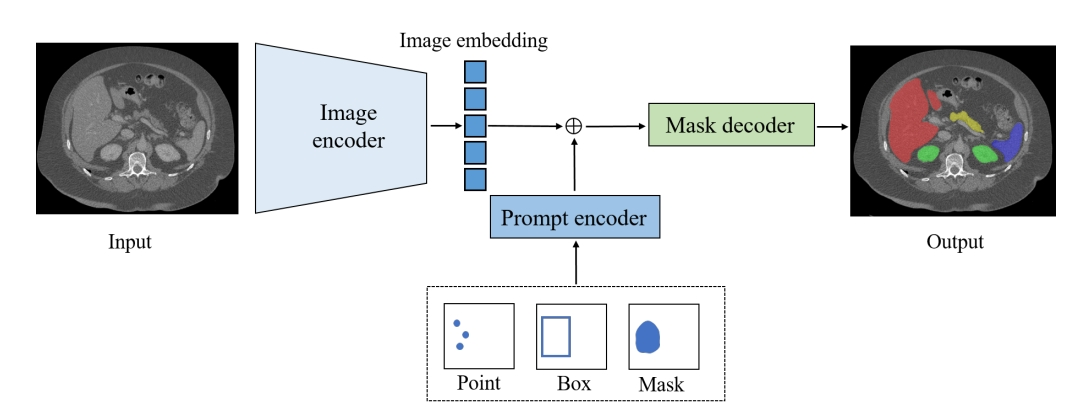
\includegraphics[width=1\textwidth]{1.jpeg}
			
			\label{fig:fig1}
			
			
		\end{figure}
		
		
		
		A\'un cuando es evidente el potencial de SAM para la segmentaci\'on de imagenes naturales, preseneta limitaciones en el \'ambito de las im\'agenes m'edicas. El rendimiento limitado de SAM en imágenes médicas se atribuye a su insuficiente comprensión de desafíos específicos del ámbito médico \parencite{Ma2023}, como el bajo contraste de imagen, los contornos de tejidos ambiguos y las pequeñas regiones de lesiones. Estos factores complican el proceso de segmentación en comparación con las imágenes naturales.
		\\
		El enfoque más avanzado para mejorar SAM para aplicaciones médicas implica realizar un ajuste completo del modelo en conjuntos de datos médicos. Sin embargo, este método es costoso en términos computacionales y requiere una cantidad significativa de recursos de memoria, lo que plantea dudas sobre su necesidad, dado que estudios previos han demostrado que los modelos visuales preentrenados suelen mostrar una fuerte transferibilidad a imágenes médicas \parencite{Raghu2019}. 
		
		En Zhang et al. \cite{Zhang2024SegmentAnything} realizan una evaluacion de SAM centrándose en una amplia gama de objetivos anatómicos y patológicos a través de diferentes modalidades de imagen médica. Estas modalidades abarcan tanto imágenes médicas en 2D (por ejemplo, radiografías, patología, ultrasonido, endoscopia y colonoscopia) como imágenes médicas en 3D (por ejemplo, Tomografía Computarizada (TC), Resonancia Magnética (RM) y Tomografía por Emisión de Positrones (PET)). Presentan el uso en cero disparos de SAM en la segmentación de imágenes médicas, organizado según los formatos de las modalidades de imagen médica.
		
		\begin{figure}[h] 
			\centering
			\caption{ Resultados cuantitativos de segmentación del modelo SAM en 18 modalidades de imagen diferentes en un estudio empírico a gran escala \cite{Huang2024}. Imagen adaptada de \cite{Zhang2024SegmentAnything}}
			\includegraphics[width=1\textwidth]{3.jpeg}
			
			\label{fig:fig2}
			
			
		\end{figure}
		
		
		
		En general, SAM requiere una interacción humana sustancial para lograr un rendimiento de segmentación moderado, lo que solo requiere unos pocos puntos o indicaciones de caja delimitadora. Los resultados de la evaluación en varios conjuntos de datos indican la limitada capacidad de generalización de SAM cuando se aplica directamente a la segmentación de imágenes médicas, que varía significativamente entre diferentes conjuntos de datos y tareas. Si bien SAM demuestra un rendimiento notable comparable a los métodos SOTA\footnote{State of the Art(Estado del arte), por sus siglas en \'ingles} en la identificación de objetos bien definidos en ciertas modalidades de imagen, presenta imperfecciones o fracasos totales en situaciones más desafiantes. Esto es particularmente evidente al tratar con objetivos de segmentación que presentan bordes débiles, bajo contraste, pequeño tamaño y formas irregulares, alineándose con los hallazgos de otras investigaciones. Para la mayoría de los escenarios de segmentación de imágenes médicas, el rendimiento subóptimo de segmentación de SAM no cumple con los requisitos para aplicaciones posteriores, particularmente en algunas tareas que exigen una precisión extremadamente alta. El conjunto de datos SA-1B, los datos de entrenamiento de SAM, está compuesto principalmente por imágenes naturales con información de borde fuerte y presenta una disimilitud significativa con las imágenes médicas. En consecuencia, aplicar SAM directamente sin ajuste fino o reentrenamiento a tareas desafiantes y no vistas previamente en la segmentación de imágenes médicas puede resultar en un rendimiento limitado. Vease \cite{Zhang2024SegmentAnything}.
		
		\subsection{Adaptando SAM para im\'agenes m\'edicas.}
		
		Por estos motivos se han realizado varios estudios con el objetivo de adaptar SAM para mejorar su rendimiento en im\'agenes m\'edicas. La figura \ref{fig:fig3} ilustra las diferentes modalidades de SAM a lo largo de los a\~nos.
		\\
			\begin{figure}[h] 
				\centering
				\caption{Una breve cronología del modelo Segment Anything (SAM) \cite{kirillov2023segment} y sus variantes para la segmentación de imágenes médicas en 2023. Imagen adaptada de Zhang et al. \cite{Zhang2024SegmentAnything}}
				\includegraphics[width=1\textwidth]{2.jpeg}
				
				\label{fig:fig3}
				
				
			\end{figure}
		
			
		Para mejorar el rendimiento insatisfactorio de SAM en tareas de segmentación de imágenes médicas, un enfoque directo e intuitivo es ajustar finamente SAM con imágenes médicas, lo que incluye tanto el ajuste completo como el ajuste eficiente de parámetros. El enfoque más sencillo para adaptar SAM a la segmentación de imágenes médicas es ajustar finamente SAM directamente en la tarea específica que se tiene entre manos.
		.
		\\
		
		Hu et al. \cite{Hu2023} presenta una validación del ajuste fino de SAM para la segmentación de cáncer de piel, demostrando una mejora sustancial en la puntuación DSC, que pasó del 81.25\% al 88.79\% . Vease \cite{Zhang2024SegmentAnything}.
		MedSAM \cite{ma2023segment} es un modelo universal para la segmentación de imágenes médicas que se adapta de SAM utilizando un conjunto de datos diverso con más de un millón de pares de imágenes y máscaras de 11 modalidades. Logró puntuaciones medianas de DSC del 94.0\% al 98.4\% en tareas como hemorragia intracraneal, glioma, neumotórax y pólipos, superando a los modelos U-Net especializados. Sin embargo, enfrenta dificultades para segmentar estructuras ramificadas similares a vasos debido a la ambigüedad en los prompts de caja delimitadora y solo procesa imágenes 3D como series de cortes 2D en lugar de volúmenes.
		\\
		
		El fine-tuning eficiente en parámetros (PEFT) es un enfoque utilizado para mejorar el rendimiento de modelos de aprendizaje automático, especialmente en el contexto de modelos de lenguaje y redes neuronales. Este método se centra en ajustar solo un pequeño subconjunto de los parámetros del modelo preentrenado, lo que permite adaptar el modelo a tareas específicas sin necesidad de realizar un ajuste completo, que puede ser costoso en términos de recursos computacionales y tiempo.
		Wu et al. \cite{Wu2023} proponen el Adaptador SAM Médico (Med-SA), que mantiene los parámetros preentrenados de SAM congelados mientras integra módulos de adaptación de rango bajo (LoRA) \cite{Hu2021} en posiciones designadas. Los extensos experimentos realizados en 17 tareas de segmentación de imágenes médicas a través de 5 modalidades diferentes muestran la superioridad de Med-SA sobre SAM y métodos anteriores de estado del arte (SOTA) \cite{Zhang2024SegmentAnything}.Similarmente SAMed \cite{SaMed} aplica una estrategia de ajuste fino basada en rango bajo (LoRA) al codificador de imágenes de SAM y lo ajusta junto con el codificador de prompts y el decodificador de máscaras en conjuntos de datos etiquetados para segmentación de imágenes médicas.Además, dado que SAMed solo actualiza una pequeña fracción de los parámetros de SAM, su costo y almacenamiento son bastante marginales en su uso práctico. Existen otro muchos modelos adaptados de SAM como se aprecia en la figura \ref{fig:fig3} 
			
		
		
		
		
	
	\newpage
	
	\section{Conclusiones}
	\newpage
	
	\section{Recomendaciones}
	en la figura \ref{fig:fig1}
	\newpage
	
	\section{Bibliograf\'ia}
	\printbibliography[title={" "}]
	\newpage
	
	\section{Anexos}
	
	
\end{document}